% !TeX root = ../main.tex
% Add the above to each chapter to make compiling the PDF easier in some editors.

\chapter{Results}\label{chapter:results}
\section{Variational Auto Encoder Benchmark}\label{section:vae_benchmark}
This section presents the experimental results to analyze the \gls{VAE} performance.
The experiments primarily focus on evaluating the range of the generator in various settings, with particular attention to the Gaussian sensing matrix and sector-wise reconstruction.
In order to properly assess the range of the generators, the generative model solver without sparse offset is used.
Three primary experiments are performed.
The first experiment varies the latent dimension of the \gls{VAE}.
The second experiment assesses the effects of fine-tuning the models for specific cities.
The third experiment compares the performance of the \gls{VAE} with \gls{Lasso} under noisy and noiseless conditions.

All experiments are performed on test data or case study cities (Munich, Paris, Zurich) in the case of fine-tuning.
Due to the vast variations produced by the timely scaling factors, they are disabled in these experiments.
Additionally, the number of measurements $m$ is varied to assess the performance under different levels of available information.
Each experiment is repeated three times, and the results are averaged.

\subsection{Latent Dimension}\label{subsection:latent_dimension}
The following experiment varies the latent dimension $d \in \{256, 512, 1024, 2048\}$ to assess the impact of the latent dimension $d$ on the reconstruction performance.
No noise is used in these experiments to better compare the latent dimensions.
This experiment is only performed on the test data without Munich, Paris, and Zurich.
\begin{figure}[h!]
    \centering
    \begin{subfigure}[b]{0.49\textwidth}
        \centering
        \includegraphics[width=0.85\textwidth]{figures/06_results/vae_benchmark/effect_of_latent_dimension/effect_of_latent_dimension_relative_error.eps}
        \caption{Relative Error}
    \end{subfigure}
    \begin{subfigure}[b]{0.49\textwidth}
        \centering
        \includegraphics[width=0.85\textwidth]{figures/06_results/vae_benchmark/effect_of_latent_dimension/effect_of_latent_dimension_ssim.eps}
        \caption{SSIM}
    \end{subfigure}
    \caption{Relative Error and SSIM for Test Data Reconstructions Using VAEs with Varying Latent Dimensions Across Measurement Counts in Compressed Sensing with Gaussian Sensing Matrices}
    \label{fig:experiment_latent_dim}
\end{figure}

The results in Figure \ref{fig:experiment_latent_dim} show the clear trend that as the number of measurements increases, both the relative error decreases and \gls{SSIM} improves.
Smaller models with lower latent dimensions plateau earlier, indicating that they are unable to fully utilize the additional information provided by more measurements.
In contrast, larger models continue to improve with more measurements.

In low-information or uncertain domains, smaller models perform better due to their smaller latent space, which simplifies optimization.
However, in cases where more information is available, larger models can capture more complex structures due to their wider range of the generator.
This trend is expected, as larger latent spaces increase the representational power of the generator, but they also make the search for solutions more difficult due to the higher dimensionality of the optimization problem.
The representational error (i.e., the error that persists at high measurement counts) is smaller for larger models, as they can capture a wider range of emission fields.
Overall, the results are consistent with the findings of \textcite{CSUsingAI}.

\subsection{Fine-tuned Models vs Base Models}
In this experiment, all models are compared to their fine-tuned counterparts.
Fine-tuning is performed for the three case study cities: Munich, Paris, and Zurich.
For each city, the number of measurements is varied, and the average improvements in relative error and \gls{SSIM} are reported in Table \ref{tab:fine_tuning} for each latent dimension for emission field of the corresponding city.

\begin{table}[htb]
    \centering
    \begin{tabular}{|c|c|c|c|c|}
        \hline
        \multirow{2}{*}{} & \multirow{2}*{\begin{tabular}{c}\textbf{Latent}\\\textbf{Dimension}\end{tabular}} & \multicolumn{3}{c|}{\textbf{City}} \\
        \cline{3-5}
        & & \textbf{Munich} & \textbf{Paris} & \textbf{Zurich} \\
        \hline
        \multirow{4}*{\begin{tabular}{c}\textbf{Relative Error}\\\textbf{Improvement}\end{tabular}}
            & 256 & \textbf{+30.87\%} & \textbf{+29.83\%} & \textbf{+31.32\%} \\
            & 512 & \textbf{+30.60\%} & \textbf{+31.59\%} & \textbf{+33.39\%} \\
            & 1024 & \textbf{+24.55\%} & \textbf{+20.20\%} & \textbf{+25.73\%} \\
            & 2048 & \textbf{+14.66\%} & \textbf{+14.54\%} & \textbf{+21.73\%} \\
        \hline
        \multirow{4}{*}{\begin{tabular}{c}\textbf{SSIM}\\\textbf{Improvement}\end{tabular}}
            & 256 & \textbf{+0.02\%} & \textbf{+5.43\%} & -4.14\% \\
            & 512 & -2.54\% & \textbf{+5.71\%} & -3.69\% \\
            & 1024 & -1.67\% & \textbf{+4.03\%} & -4.61\% \\
            & 2048 & -1.63\% & \textbf{+2.10\%} & -4.53\% \\
        \hline
    \end{tabular}
    \caption{Average Improvements in Relative Error and SSIM from Fine-tuning in Reconstruction of Emissions for Munich, Paris, and Zurich}
    \label{tab:fine_tuning}
\end{table}

The general trend shows that the models with smaller latent dimensions see the most significant improvement from fine-tuning.
This makes sense because smaller models have a more limited range and are thus less likely to capture these emission fields through their generators.
Regarding \gls{SSIM}, the changes are less significant overall, with slight decreases observed for Munich and Zurich but small improvements for Paris.
The most considerable improvement in relative error is seen in Zurich.

\subsection{VAE vs Lasso}
The following experiment compares the $2048$-dimensional \gls{VAE} against \gls{Lasso}, \gls{Lasso} with \gls{DCT}, and \gls{Lasso} with \gls{DWT}, again, on the test data without the case study cities.
These comparisons are in line with the experiments conducted by \textcite{CSUsingAI}.
The number of measurements $m$ is again varied, and two sets of experiments are conducted: one with no noise and one with a \gls{SNR} of $20 \unit{dB}$.

\begin{figure}[htb]
    \centering
    \begin{subfigure}[b]{0.49\textwidth}
        \centering
        \includegraphics[width=0.85\textwidth]{figures/06_results/vae_benchmark/vae_vs_lasso/vae_vs_lasso_relative_error.eps}
        \caption{Relative Error (no noise)}
    \end{subfigure}
    \begin{subfigure}[b]{0.49\textwidth}
        \centering
        \includegraphics[width=0.85\textwidth]{figures/06_results/vae_benchmark/vae_vs_lasso/vae_vs_lasso_ssim.eps}
        \caption{SSIM (no noise)}
    \end{subfigure}
    \begin{subfigure}[b]{0.49\textwidth}
        \centering
        \includegraphics[width=0.85\textwidth]{figures/06_results/vae_benchmark/vae_vs_lasso/vae_vs_lasso_relative_error_noisy.eps}
        \caption{Relative Error ($\text{SNR} = 20 \unit{dB}$)}
    \end{subfigure}
    \begin{subfigure}[b]{0.49\textwidth}
        \centering
        \includegraphics[width=0.85\textwidth]{figures/06_results/vae_benchmark/vae_vs_lasso/vae_vs_lasso_ssim_noisy.eps}
        \caption{SSIM ($\text{SNR} = 20 \unit{dB}$)}
    \end{subfigure}
    \caption{Relative Error and SSIM of Test Data Reconstructions Using VAE (2048) and Lasso with Various Basis Transforms Across Measurement Counts in Compressed Sensing with Gaussian Sensing Matrices}
    \label{fig:results_vae_vs_lasso}
\end{figure}

The results in Figure \ref{fig:results_vae_vs_lasso} indicate that the \gls{VAE} outperforms all variations of \gls{Lasso} when the number of measurements is low.
This is particularly true for \gls{SSIM}, where the \gls{VAE} performs better until around $5 \cdot 10^{3}$ to $10 \cdot 10^{3}$ measurements.
In the noisy case, the \gls{VAE} is less affected by the noise, which makes sense because noisy representations are less likely to be found within the range of the generator and, therefore, cannot be generated by it.
Beyond approximately $5 \cdot 10^{3}$ measurements, the \gls{VAE}'s improvement saturates, indicating that the optimization of the latent variables is complete, while all variants of \gls{Lasso} keep improving and outperforming the \gls{VAE} significantly.
At this point, the error of the \gls{VAE} is mainly the representational error of the model.
The significant difference between \gls{Lasso} and the \gls{VAE} indicates that much improvement needs to be made in terms of the generative capabilities of the \gls{VAE}.

\section{Atmospheric Inversion}\label{section:atmospheric_inversion_results}
This section presents the results of the \gls{VAE} applied to the atmospheric inversion problem as defined in Subsection \ref{subsec:atmospheric_inversion}.
This section uses the generative model solver with sparse offset to achieve optimal performance.
All experiments were conducted on the three case study cities.

Two types of experiments were conducted.
The first explores the effect of varying \gls{SNR} while keeping the number of measurements fixed.
The second focuses on a qualitative case study of Munich, providing visual insights into the \gls{VAE}'s reconstruction capabilities.

\subsection{Atmospheric Inversion for Different SNR Levels}
In the first experiment, artificial footprints by \textcite{UrbanSparseReconstructionFootprints} are used to maintain consistency with prior work.
The experimental setup includes $3\%$ measurement stations relative to the number of unknowns, corresponding to $30$ stations in this case.
Each measurement station takes $50$ measurements, resulting in a total of $1500$.
The primary variable in this experiment is the \gls{SNR}, and each experiment was repeated three times to ensure robustness, with results averaged accordingly.
Results are reported separately for Munich, Zurich, and Paris.
The \gls{VAE} used had a latent dimension $d = 2048$, as this configuration showed the best performance for the given setup.

\begin{figure}[htb]
    \centering
    \begin{subfigure}[b]{0.49\textwidth}
        \centering
        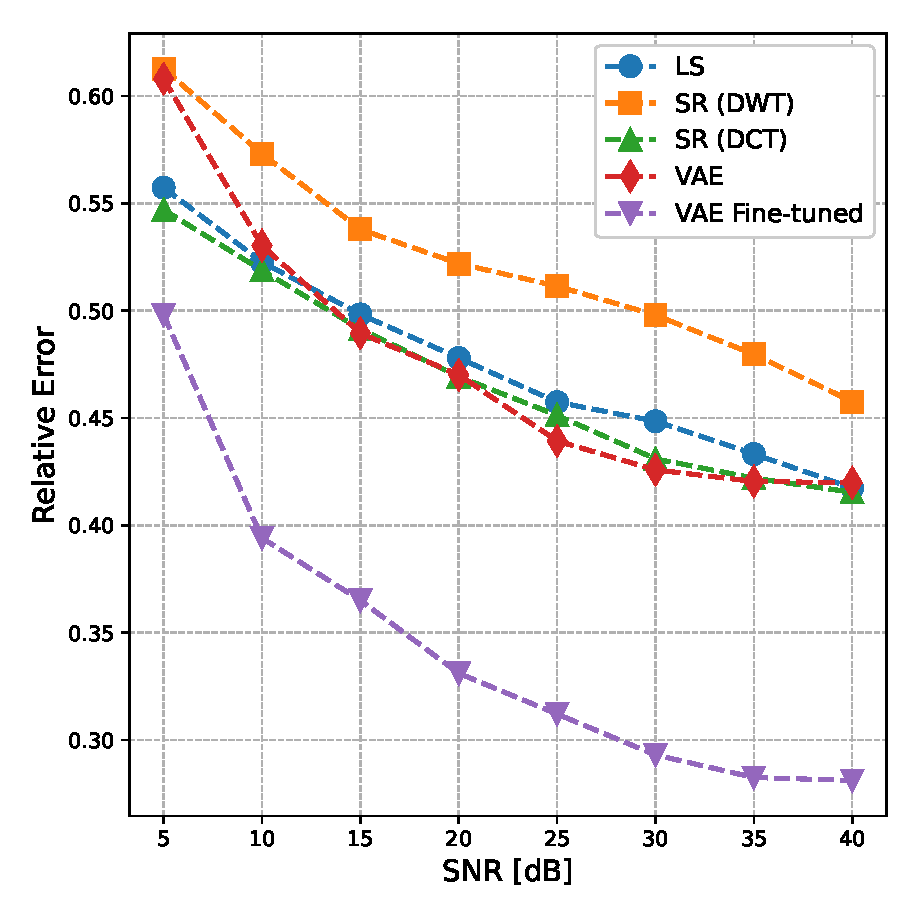
\includegraphics[width=0.85\textwidth]{figures/06_results/snr_plots/munich_relative_error.eps}
        \caption{Relative Error}
        \label{subfig:munich_results_relative_error}
    \end{subfigure}
    \begin{subfigure}[b]{0.49\textwidth}
        \centering
        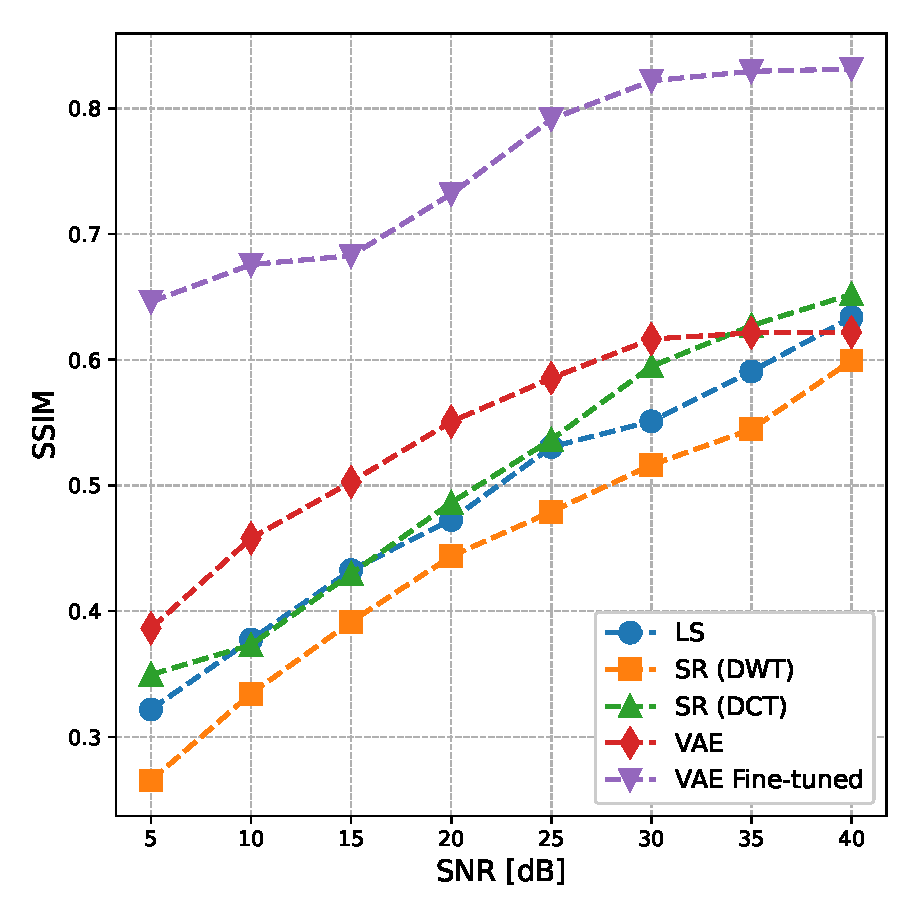
\includegraphics[width=0.85\textwidth]{figures/06_results/snr_plots/munich_ssim.eps}
        \caption{SSIM}
    \end{subfigure}
    \caption{Relative Error and SSIM for Atmospheric Inversion of Munich 2018 Emissions Across Different Solvers and SNR Levels}
    \label{fig:munich_results}
\end{figure}

The results for Munich in Figure \ref{fig:munich_results} indicate that the fine-tuned model outperforms all other solvers significantly in terms of both relative error and \gls{SSIM}.
Notably, the generative model excels in terms of \gls{SSIM}, demonstrating its capability to reconstruct spatial features.
Even the base \gls{VAE} model shows competitive performance, surpassing \gls{LS} and \gls{BPDN} at low \gls{SNR} levels with respect to \gls{SSIM}.
However, the \gls{VAE} appears more sensitive to noise, which is evident in its more substantial decline in relative error and \gls{SSIM} compared to the other solvers with decreasing \gls{SNR} levels.

% \begin{itemize}
%     \item fine-tuned model performs siginificantly better in terms of relative error and SSIM than all other solvers
%     \item especially in terms of SSIM the generative models seems to perform better
%     \item even the base model shows competetive performance, outperforming all other models at low SNR in terms of SSIM
%     \item however, it seems that the sparse models are more effected by noise, as seen in the very low SNR values
% \end{itemize}

\begin{figure}[htb]
    \centering
    \begin{subfigure}[b]{0.49\textwidth}
        \centering
        \includegraphics[width=0.85\textwidth]{figures/06_results/snr_plots/zürich_relative_error.eps}
        \caption{Relative Error}
    \end{subfigure}
    \begin{subfigure}[b]{0.49\textwidth}
        \centering
        \includegraphics[width=0.85\textwidth]{figures/06_results/snr_plots/zürich_ssim.eps}
        \caption{SSIM}
    \end{subfigure}
    \caption{Relative Error and SSIM for Atmospheric Inversion of Zurich 2018 Emissions Across Different Solvers and SNR Levels}
    \label{fig:zurich_results}
\end{figure}

The results for Zurich in Figure \ref{fig:zurich_results} follow a similar trend to those observed in Munich, with the fine-tuned model demonstrating superior performance across both metrics for all noise levels.
The base model performs comparably to the \gls{LS} and \gls{BPDN} methods employing \gls{DCT}.
However, its performance is again affected at higher noise levels, as LS shows lower relative error than the base \gls{VAE} for \gls{SNR} levels of $5 \unit{dB}$ and $10 \unit{dB}$.

\begin{figure}[htb]
    \centering
    \begin{subfigure}[b]{0.49\textwidth}
        \centering
        \includegraphics[width=0.85\textwidth]{figures/06_results/snr_plots/paris_relative_error.eps}
        \caption{Relative Error}
    \end{subfigure}
    \begin{subfigure}[b]{0.49\textwidth}
        \centering
        \includegraphics[width=0.85\textwidth]{figures/06_results/snr_plots/paris_ssim.eps}
        \caption{SSIM}
    \end{subfigure}
    \caption{Relative Error and SSIM for Atmospheric Inversion of Paris 2018 Emissions Across Different Solvers and SNR Levels}
    \label{fig:paris_results}
\end{figure}

The results for Paris in Figure \ref{fig:paris_results} deviate from those observed in Munich and Zurich.
Compared to all other solvers at all noise levels, the base \gls{VAE} model exhibits the poorest relative error, with an \gls{SSIM} that is only on par with \gls{BPDN} with \gls{DWT}.
Furthermore, while the fine-tuned \gls{VAE}s show superior results for Munich and Zurich compared to all other solvers, the results for Paris are different.
In particular, the fine-tuned \gls{VAE} barely manages to close the relative error and \gls{SSIM} gap to \gls{BPDN} with \gls{DCT}.

\subsection{Case Study: Munich}
The second atmospheric inversion experiment is performed using the Munich emission field from $2018$, with $13$ measurement stations randomly placed around the city.
Each measurement station collects $50$ measurements, resulting in $650$ observations.
The corresponding footprints are generated using Gaussian plume simulations.
The artificial wind field used in the simulations covers approximately $180$ degrees.
Measurements are taken once at a low to moderate \gls{SNR} of $20 \unit{dB}$ and once at a higher \gls{SNR} of $5 \unit{dB}$.

The results for all solvers are shown in Table \ref{tab:case_study_munich}.
The table reports the relative error and the \gls{SSIM} for each solver.
Additionally, a visual representation of the reconstructed emission flux fields for the best solvers is presented in Figure \ref{fig:example_munich_20_dB} for $\text{\gls{SNR} = 20 \unit{dB}}$ and in Figure \ref{fig:example_munich_5_dB} for $\text{\gls{SNR} = 5 \unit{dB}}$.
Overall, the \gls{SSIM} reflects well the visual similarity of each reconstruction with the target emissions.

\begin{table}[htb]
    \centering
    \begin{tabular}{|l|c|c|c|c|}
        \hline
        \multirow{2}{*}{\textbf{Solver}} & \multicolumn{2}{c|}{\textbf{\gls{SNR} = 20dB}} & \multicolumn{2}{c|}{\textbf{\gls{SNR} = 5dB}} \\
        \cline{2-5}
        & \textbf{Relative Error} & \textbf{SSIM} & \textbf{Relative Error} & \textbf{SSIM} \\
        \hline
        \hline
        \gls{VAE} (256) & 55.117\% & 0.421 & 71.153\% & 0.322 \\
        \gls{VAE} (512) & 50.818\% & 0.459 & 70.760\% & 0.320 \\
        \gls{VAE} (1024) & 49.037\% & 0.477 & 70.753\% & 0.295 \\
        \gls{VAE} (2048) & 44.791\% & 0.563 & 78.960\% & 0.371 \\
        \hline
        \gls{VAE} (256) Fine-tuned & 46.125\% & 0.565 & 56.808\% & 0.478 \\
        \gls{VAE} (512) Fine-tuned & 36.888\% & 0.674 & 52.241\% & 0.496 \\
        \gls{VAE} (1024) Fine-tuned & 34.988\% & 0.739 & 53.035\% & 0.521 \\
        \textbf{\gls{VAE} (2048) Fine-tuned} & \textbf{31.766\%} & \textbf{0.747} & \textbf{51.201\%} & \textbf{0.585} \\
        \hline
        BPDN (DWT) & 49.867\% & 0.466 & 63.282\% & 0.273 \\
        BPDN (DCT) & 48.475\% & 0.501 & 53.981\% & 0.351 \\
        \hline
        LS & 50.065\% & 0.429 & 57.817\% & 0.298 \\
        \hline
    \end{tabular}
    \caption{Relative Error and SSIM for 2018 Munich Emission Estimation after Atmospheric Inversion Using Different Solvers}
    \label{tab:case_study_munich}
\end{table}

Focusing on the experiment with $\text{\gls{SNR} = 20 \unit{dB}}$, a few key observations can be made.
The performance of the \gls{VAE}s improves as the latent dimension $d$ increases.
This is true for both the base and fine-tuned models.
This indicates that enough information is present in the measurements to saturate the optimization of the latent variables even at $d = 2048$.
Overall, the fine-tuned \gls{VAE}s show, by far, the best reconstruction quality.
Thus, the overall best-performing model is the fine-tuned \gls{VAE} with $d=2048$.
However, even the base \gls{VAE}s show good reconstruction results here, with the base \gls{VAE} with $d=2048$ outperforming both \gls{BPDN} variants and \gls{LS} regarding the relative error and \gls{SSIM}.
When ignoring the \gls{VAE}s with smaller latent dimensions, the \gls{LS} approach emerges as the worst reconstruction technique in this experiment, with the highest relative error and lowest \gls{SSIM}.
This also highlights the strengths of sparse reconstruction and its ability to reconstruct emissions with fewer measurements than \gls{LS}, as shown by \textcite{UrbanSparseReconstruction}, even when the underlying emission field is not very sparse.

Now, focusing on the experiment with $\text{\gls{SNR} = 20 \unit{dB}}$, the results are not as straightforward.
As expected, every solver performs worse, with a higher relative error and lower \gls{SSIM}.
It can be observed that the \gls{BPDN} and \gls{LS} solvers are heavily impacted in their \gls{SSIM} while the \gls{VAE}s are more impacted in terms of relative error.
This steep decline of the \gls{VAE}s in the relative error is in line with results in Figure \ref{subfig:munich_results_relative_error}.
Percentage-wise, the base \gls{VAE}s with higher latent dimensions are impacted more strongly than those with smaller dimensions.
This can be explained by their larger range, which makes them more susceptible to reconstruction errors.
While the fine-tuned models again improve with bigger latent dimensions, the base \gls{VAE}s do not see this improvement.
For instance, the \gls{VAE} with $d = 2048$ has a much higher relative error than the \gls{VAE} with $d = 256$. 
This indicates that the optimization is not able to effectively use the given information in the search for reconstruction samples in the latent space.
This is different for the fine-tuned models, as their range, which covers the Munich emissions better, can guide the optimizer to solutions that are close to the target.
The base \gls{VAE}s have the most significant relative error, but the second-best \gls{SSIM} at $d = 2048$ behind the fine-tuned VAEs.

% \begin{table}[htb]
%     \centering
%     \begin{tabular}{|l|c|c|}
%         \hline
%         \textbf{Solver} & \textbf{Relative Error ($\text{\gls{SNR}} = 20 \unit{dB}$)} & \textbf{SSIM} \\
%         \hline
%         \hline
%         \gls{VAE} (256) & 54.880\% & 0.426 \\
%         \gls{VAE} (512) & 50.999\% & 0.499 \\
%         \gls{VAE} (1024) & 48.941\% & 0.493 \\
%         \gls{VAE} (2048) & 46.139\% & 0.520 \\
%         \hline
%         \gls{VAE} (256) Fine-tuned & 46.333\% & 0.585 \\
%         \gls{VAE} (512) Fine-tuned & 35.974\% & 0.710 \\
%         \gls{VAE} (1024) Fine-tuned & 37.609\% & 0.739 \\
%         \textbf{\gls{VAE} (2048) Fine-tuned} & \textbf{32.833\%} & \textbf{0.751} \\
%         \hline
%         BPDN (DWT) & 51.102\% & 0.445 \\
%         BPDN (DCT) & 47.767\% & 0.514 \\
%         \hline
%         LS & 49.767\% & 0.449 \\
%         \hline
%     \end{tabular}
%     \caption{Relative Error and SSIM for Different Solvers}
%     \label{tab:case_study_munich}
% \end{table}

\begin{figure}[htb]
    \centering
    \begin{minipage}[b]{\textwidth}
        \centering
        \begin{subfigure}[b]{0.32\textwidth}
            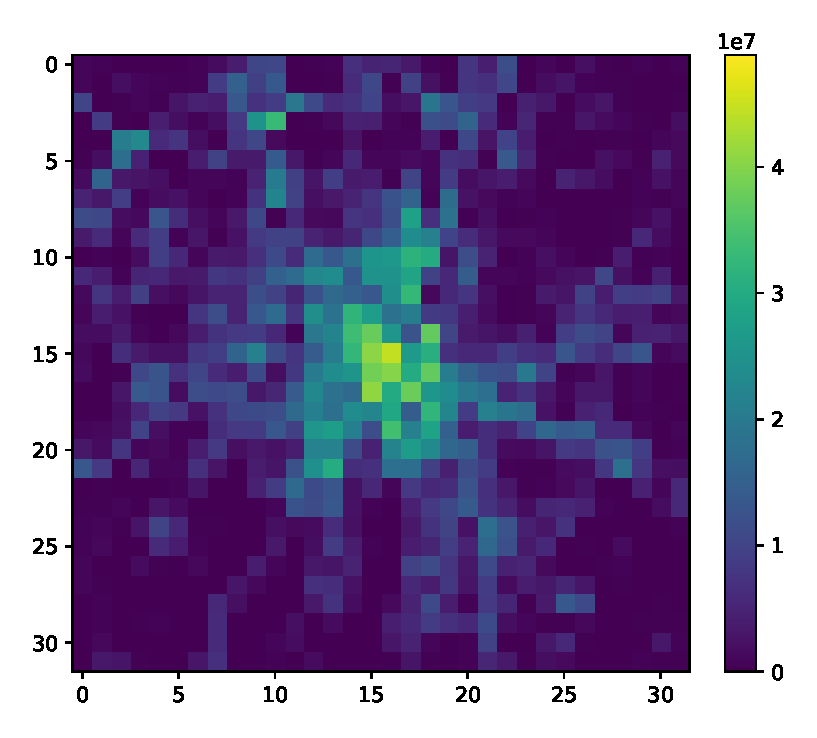
\includegraphics[width=\textwidth]{figures/06_results/gaussian_plume_example/munich/target.eps}
            \caption{Target Emissions}
        \end{subfigure}
        \begin{subfigure}[b]{0.32\textwidth}
            \includegraphics[width=\textwidth]{figures/06_results/gaussian_plume_example/munich/gen_2048_fine_tuned_snr_20_db.eps}
            \caption{\gls{VAE} (2048) Fine-tuned}
        \end{subfigure}
        \begin{subfigure}[b]{0.32\textwidth}
            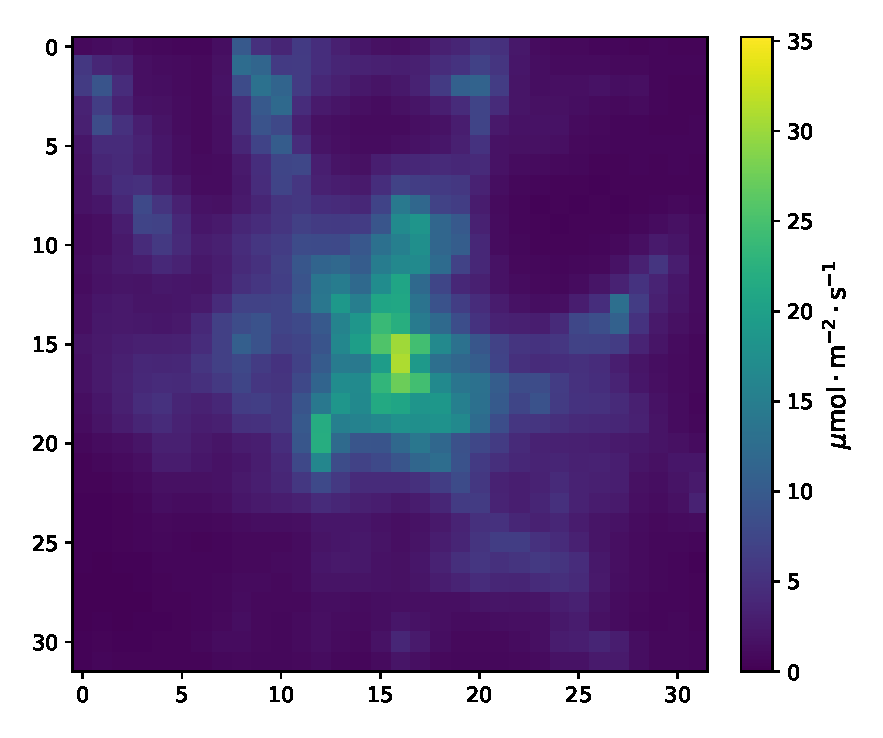
\includegraphics[width=\textwidth]{figures/06_results/gaussian_plume_example/munich/gen_2048_snr_20_db.eps}
            \caption{\gls{VAE} (2048)}
        \end{subfigure}
        \begin{subfigure}[b]{0.32\textwidth}
            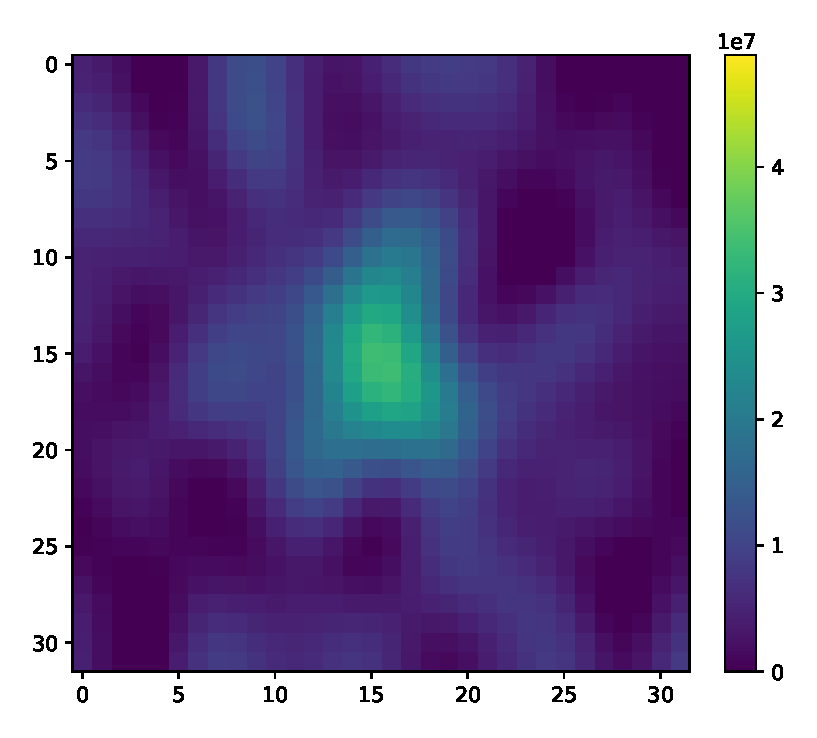
\includegraphics[width=\textwidth]{figures/06_results/gaussian_plume_example/munich/bp_dct_snr_20_db.eps}
            \caption{BPDN (DCT)}
        \end{subfigure}    
        \begin{subfigure}[b]{0.32\textwidth}
            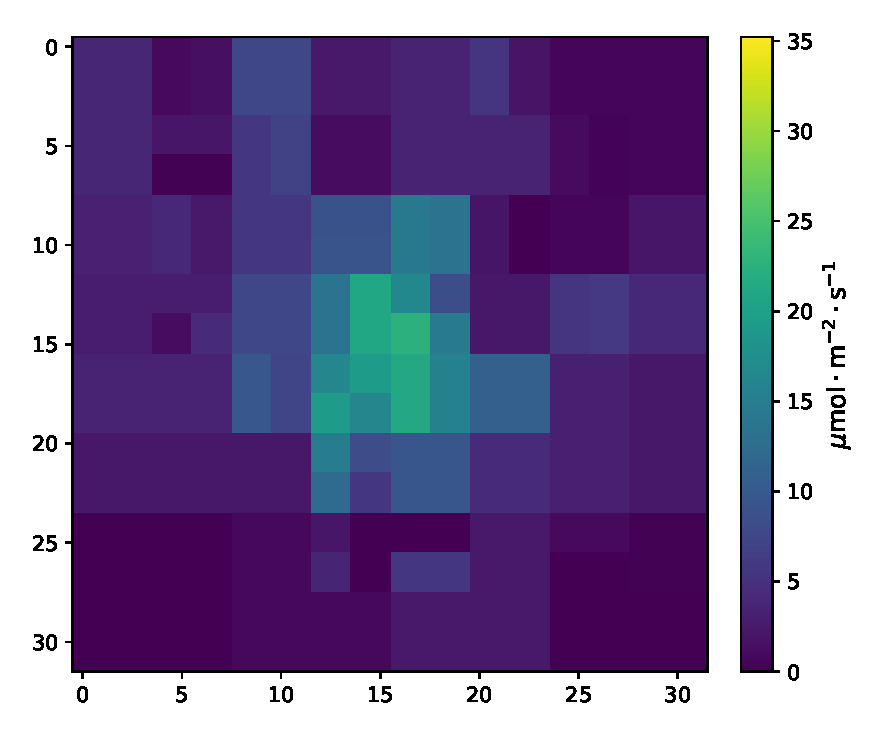
\includegraphics[width=\textwidth]{figures/06_results/gaussian_plume_example/munich/bp_dwt_snr_20_db.eps}
            \caption{BPDN (DWT)}
        \end{subfigure}
        \begin{subfigure}[b]{0.32\textwidth}
            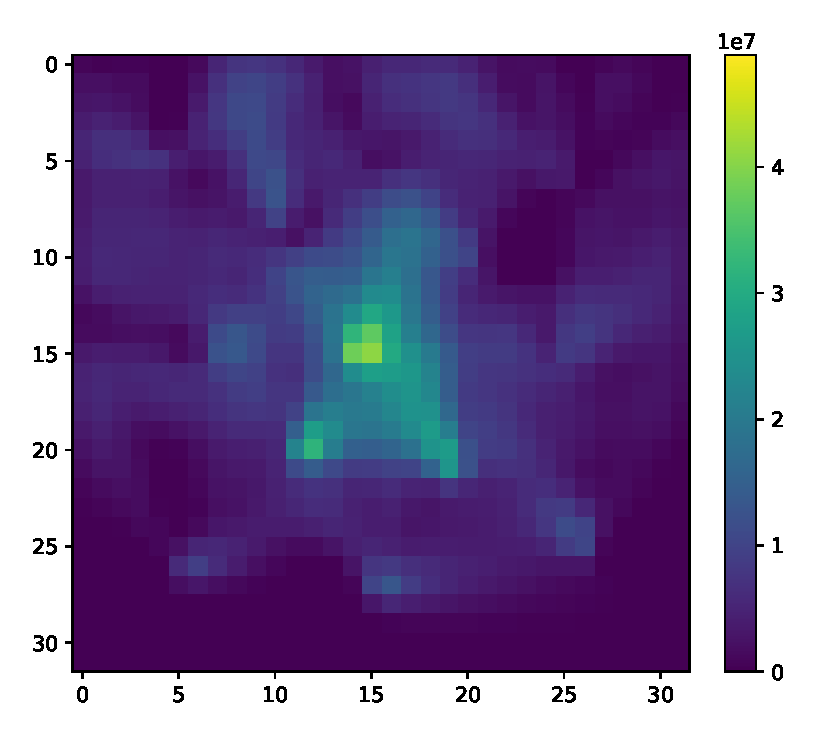
\includegraphics[width=\textwidth]{figures/06_results/gaussian_plume_example/munich/least_squares_snr_20_db.eps}
            \caption{LS}
        \end{subfigure}
        \caption{Estimated 2018 Munich Emission Flux Fields after Atmospheric Inversion with Different Solvers at SNR = 20dB}
        \label{fig:example_munich_20_dB}
    \end{minipage}
    \begin{minipage}[b]{\textwidth}
        \centering
        \begin{subfigure}[b]{0.32\textwidth}
            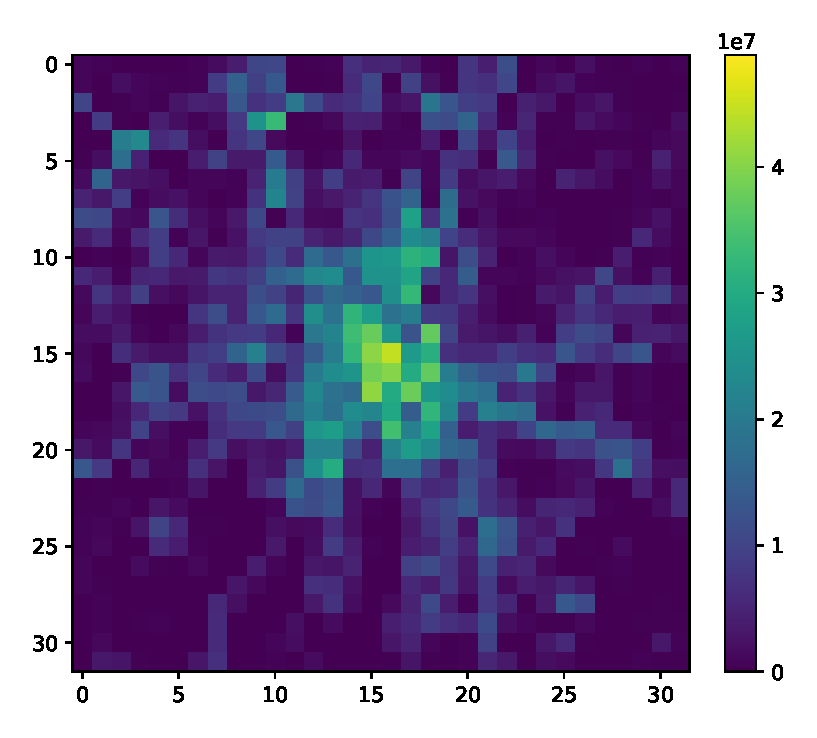
\includegraphics[width=\textwidth]{figures/06_results/gaussian_plume_example/munich/target.eps}
            \caption{Target Emissions}
        \end{subfigure}
        \begin{subfigure}[b]{0.32\textwidth}
            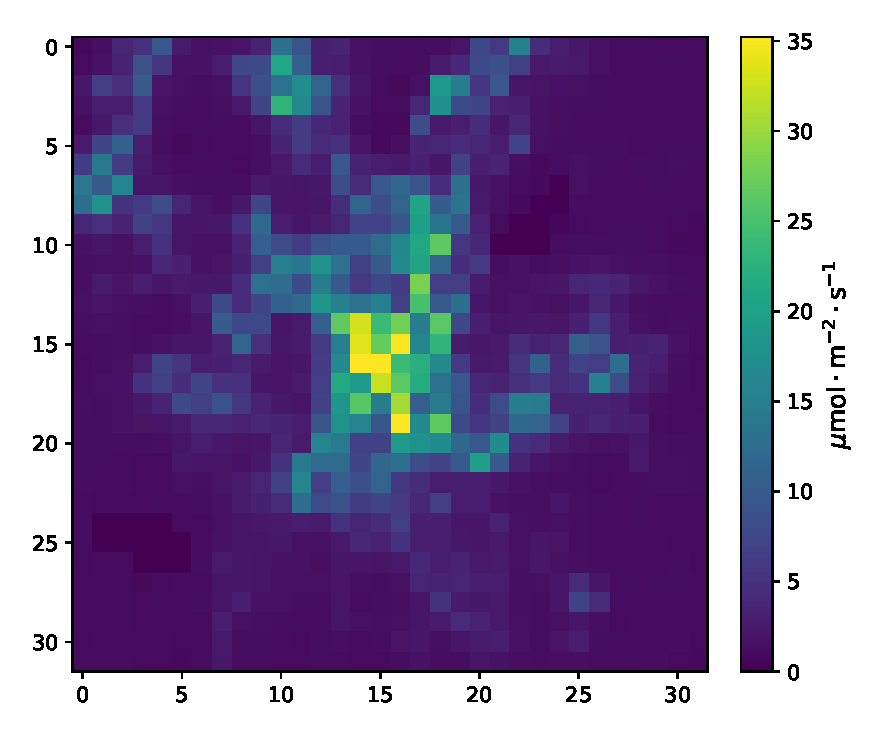
\includegraphics[width=\textwidth]{figures/06_results/gaussian_plume_example/munich/gen_2048_fine_tuned_snr_5_db.eps}
            \caption{\gls{VAE} (2048) Fine-tuned}
        \end{subfigure}
        \begin{subfigure}[b]{0.32\textwidth}
            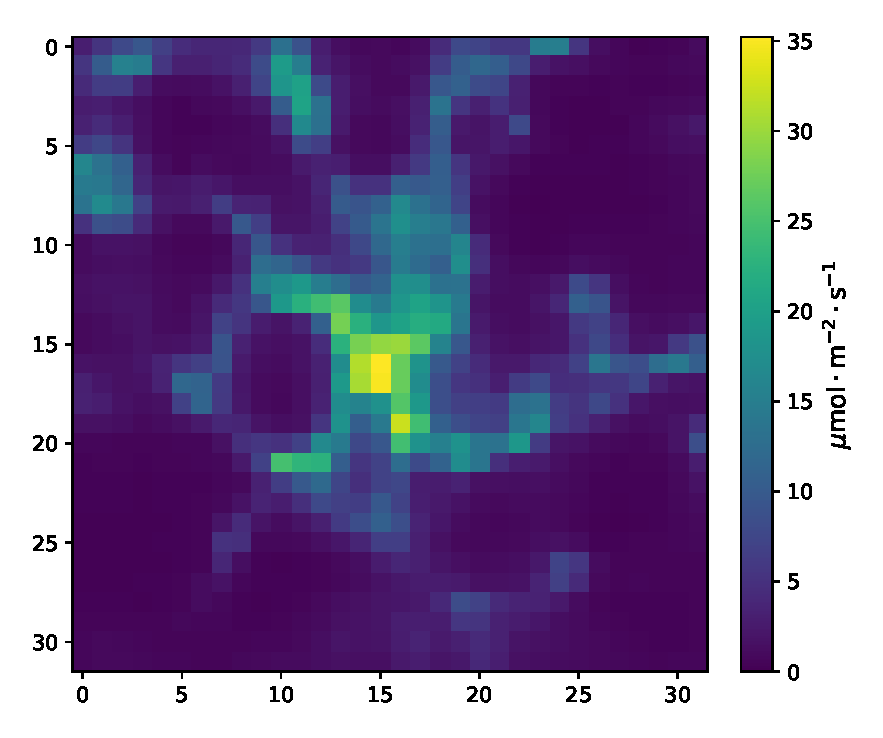
\includegraphics[width=\textwidth]{figures/06_results/gaussian_plume_example/munich/gen_512_snr_5_db.eps}
            \caption{\gls{VAE} (512)}
        \end{subfigure}
        \begin{subfigure}[b]{0.32\textwidth}
            \includegraphics[width=\textwidth]{figures/06_results/gaussian_plume_example/munich/bp_dct_snr_5_db.eps}
            \caption{BPDN (DCT)}
        \end{subfigure}    
        \begin{subfigure}[b]{0.32\textwidth}
            \includegraphics[width=\textwidth]{figures/06_results/gaussian_plume_example/munich/bp_dwt_snr_5_db.eps}
            \caption{BPDN (DWT)}
        \end{subfigure}
        \begin{subfigure}[b]{0.32\textwidth}
            \includegraphics[width=\textwidth]{figures/06_results/gaussian_plume_example/munich/least_squares_snr_5_db.eps}
            \caption{LS}
        \end{subfigure}
        \caption{Estimated 2018 Munich Emission Flux Fields after Atmospheric Inversion with Different Solvers at SNR = 5dB}
        \label{fig:example_munich_5_dB}
    \end{minipage}
\end{figure}

Overall, this case study represents how difficult the atmospheric inversion task without accurate priors is.
All solvers struggle to achieve a relative error of below $30\%$ and \gls{SSIM} beyond $0.75$, even in a low to moderate noise scenario.
